%----------------------------------------------------------------------------------------
%	PACKAGES AND DOCUMENT CONFIGURATIONS
%----------------------------------------------------------------------------------------

\documentclass[a4paper]{report}
\usepackage[utf8]{inputenc}
\usepackage[italian]{babel}
\usepackage{microtype}
\usepackage{appendix}
\usepackage{csquotes}
\usepackage{geometry}
\usepackage[T1]{fontenc}
\usepackage{siunitx} % Provides the \SI{}{} and \si{} command for typesetting SI units
\usepackage{graphicx} % Required for the inclusion of images
\usepackage{natbib} % Required to change bibliography style to APA
\usepackage{amsmath} % Required for some math elements 
\usepackage{caption}
\usepackage{tikz}
\usepackage{pdfpages}
\usepackage{graphicx}
\usepackage{float}
\usepackage[hidelinks]{hyperref}

\usetikzlibrary{arrows,automata, positioning}
\tikzset{
  ->, % makes the edges directed
  >=stealth', % makes the arrow heads bold
  node distance=4.1cm, % specifies the minimum distance between two nodes. Change if necessary.
  every state/.style={thick, fill=gray!10}, % sets the properties for each ’state’ node
  initial text=$ $, % sets the text that appears on the start arrow
}

\usepackage{import}

%----------------------------------------------------------------------------------------
%	DOCUMENT INFORMATION
%----------------------------------------------------------------------------------------

\title{Prova Finale di Reti Logiche} % Title
\author{Leonardo Airoldi} % Author name
\date{A. A. 2021-22}

\begin{document}
\maketitle % Insert the title, author and date


\tableofcontents
\newpage



% If you wish to include an abstract, uncomment the lines below
% \begin{abstract}
% Abstract text
% \end{abstract}

%----------------------------------------------------------------------------------------
%	INTRODUZIONE
%----------------------------------------------------------------------------------------

\chapter{Introduzione}


La specifica della Prova finale (Progetto di Reti Logiche) 2021 richiede di implementare un \textbf{codificatore convoluzionale} usando il linguaggio VHDL.\\
Un codificatore convoluzionale è un dispositivo che tramite l'applicazione di un \textit{codice convoluzionale} codifica uno stream di bit in ingresso in uno stream di bit in uscita ridondante che permette a un dispositivo che legge lo stream codificato di risalire allo stream originale anche in presenza di errori applicando tecniche di \textit{error-correction}.
Codificatori convoluzionali elettronici sono molto comuni nell'ambito delle telecomunicazioni, in quanto conferiscono a una rete un certo grado di robustezza: un dispositivo ricevente può ricostruire il segnale trasmesso, che potrebbe risultare corrotto a causa del rumore sulla linea, senza richiedere un ulteriore invio dell'informazione.

\section{Specifiche}
Nel caso specifico di questo progetto, è richiesto lo sviluppo di un circuito integrato con le seguenti caratteristiche: 
\begin{enumerate}
\item il \textit{codice convoluzionale} ha \textbf{tasso di trasmissione} $\frac{1} {2}$.
\item si interfaccia con una memoria sincrona a word di 8bit e indirizzi a 16bit.
\item lo stream in ingresso è di dimensione $n$ words memorizzate a partire dall'indirizzo \texttt{0x01}.
\item la dimensione dello stream è memorizzata all'indirizzo \texttt{0x00} ed è al massimo di 255 word.
\item il dispositivo viene sempre inizializzato con un segnale di \texttt{reset}.
\item la computazione inizia al segnale di \texttt{start} e termina quando il dispositivo alza il segnale \texttt{done}. Il dispositivo deve essere in grado di gestire computazioni successive senza aver bisogno di un segnale di \texttt{reset}. Si presuppone che il segnale di \texttt{start} rimanga alto durante tutta la computazione e che non possa essere rialzato prima che il segnale di \texttt{done} sia stato riportato a \texttt{0}.
\item il dispositivo deve funzionare con un periodo di clock di almeno \texttt{100ns}
\end{enumerate}

\section{Strumenti}
Il progetto sarà sviluppato in \textbf{VHDL} (VHSIC Hardware Description Language) che permette di descrivere circuiti integrati.
Per la simulazione e la sintesi della scheda il software utilizzato è \textbf{Xilinx Vivado} (\textit{v2021.1}).
Il dispositivo sarà poi implementato su una \textbf{FPGA Artix 7 \texttt{xc7a200tfbg484-1}}.

\section{Esempio}
Si prenda in analisi un caso di utilizzo caratterizzato da 3 elaborazioni richieste alla macchina in sequenza, dove la seconda è avviata a 1000ns dal termine della prima tramite il segnale \textit{start} e la terza viene interrotta dopo un \textit{reset} del dispositivo e riavviata.

Il circuito deve essere in grado di elaborare correttamente tutti i 3 i segnali presenti nella RAM durante le 3 elaborazioni, partendo solamente dopo il segnale di start e segnalando la fine di ciascuna con un segnale di \textit{done}, mantenuto alzato fino a che il segnale di start non è riportato a 0.

\subsubsection{Elaborazione 1}
Prima di ogni primo utilizzo il reset della macchina è alzato. In questo caso viene alzato per 100ns e dopo altri 100ns di attesa viene richiesto lo start dell'elaborazione. Questa elaborazione consiste in uno stream di solo 2 byte. Al termine di questa elaborazione lo start viene abbassato solo 500ns dopo la segnalazione di done da parte della macchina. \textit{done} dovrà dunque rimanere 1.
\begin{verbatim}
RAM Input data
[0] 2
[1] 162
[2] 75

RAM Expected output
[1000] 209    [1001] 205
[1002] 247    [1003] 210
\end{verbatim}

\subsubsection{Elaborazione 2}
Dopo la prima elaborazione vengono lasciati 1000ns di attesa, dopo i quali viene segnalato un nuovo start. In questa elaborazione viene computato uno stream di 6 byte.
\begin{verbatim}
RAM Input data
[0] 6
[1] 163
[2] 47
[3] 4
[4] 64
[5] 67
[6] 13
  
RAM Expected output
[1000] 209    [1001] 206
[1002] 189    [1003] 37
[1004] 176    [1005] 55
[1006] 55     [1007] 0
[1008] 55     [1009] 14
[1010] 176    [1011] 232
\end{verbatim}

\subsubsection{Elaborazione 3}
La terza elaborazione comuncia 100ns dopo la prima ma a 500ns dalla partenza, il segnale di reset si alza per 10ns. La macchina dovrebbe comportarsi correttamente e resettare il proprio stato. Un nuovo segnale di start viene quindi dato 500 ns dopo il reset: a questo punto l'elaborazione dovrebbe ricominciare e terminare correttamente.
\begin{verbatim}
RAM Input data
[0] 3
[1] 112
[2] 164
[3] 45
  
RAM Expected output
[1000] 57     [1001] 176
[1002] 209    [1003] 247
[1004] 13     [1005] 40
\end{verbatim}

%----------------------------------------------------------------------------------------
%	ARCHITETTURA
%----------------------------------------------------------------------------------------

\chapter{Architettura}
Il dispositivo è stato implementato come una macchina a stati che controlla un datapath, che si interfaccia con diversi componenti più piccoli. La scelta di dividere il progetto moduli più piccoli è stata presa per non rendere troppo complessa e articolata la gestione del dispositivo nella sua interezza. In questo modo la macchina a stati si limita a gestire la comunicazione e coordinazione dei vari componenti, che eseguono ciascuno una funzione definita anch'essa da una macchina a stati interna.

\section{Serializzatore}

Il \textbf{serializzatore} è il componente addetto alla serializzazione in un flusso continuo di bit dei byte caricati dalla ram.
Il serializzatore si interfaccia, oltre al segnale di \textit{clock} e al segnale di \textit{reset}, con il segnale di ingresso da serializzare \texttt{[input:8bit]} e dal segnale di controllo \textit{start}. Produce in uscita un segnale di \texttt{[output:1bit]} che corrisponde al flusso serializzato del byte in input e un segnale di \textit{done} che indica la fine della serializzazione.

Al segnale di \texttt{start} della serializzazione il componente passa dallo stato \texttt{STOPPED} allo stato attivo. Quando il componente è attivo produce in uscita per \textbf{due clicli di clock} l'\textit{n-esimo} bit del segnale in ingresso, incrementando poi il contatore per produrre in uscita l'\textit{n+1 esimo} bit del byte in ingresso nei prossimi due cicli di clock. La serializzazione termina quando il contatore interno raggiunge il valore \texttt{111}: il registro viene incrementato tornando quindi a \texttt{0} ma il serializzatore torna nello stato \texttt{STOPPED}, che alza il segnale di \texttt{done} a \texttt{1}.

Il flusso in uscita ha periodo di due cicli di clock in quanto al convolutore server produrre due bit sequenzialmente in uscita per ogni bit in entrata. In questo modo la velocità di serializzazione è ridotta della metà ma il convolutore riesce a produrro il flusso risultante sullo stesso ciclo di clock della macchina.

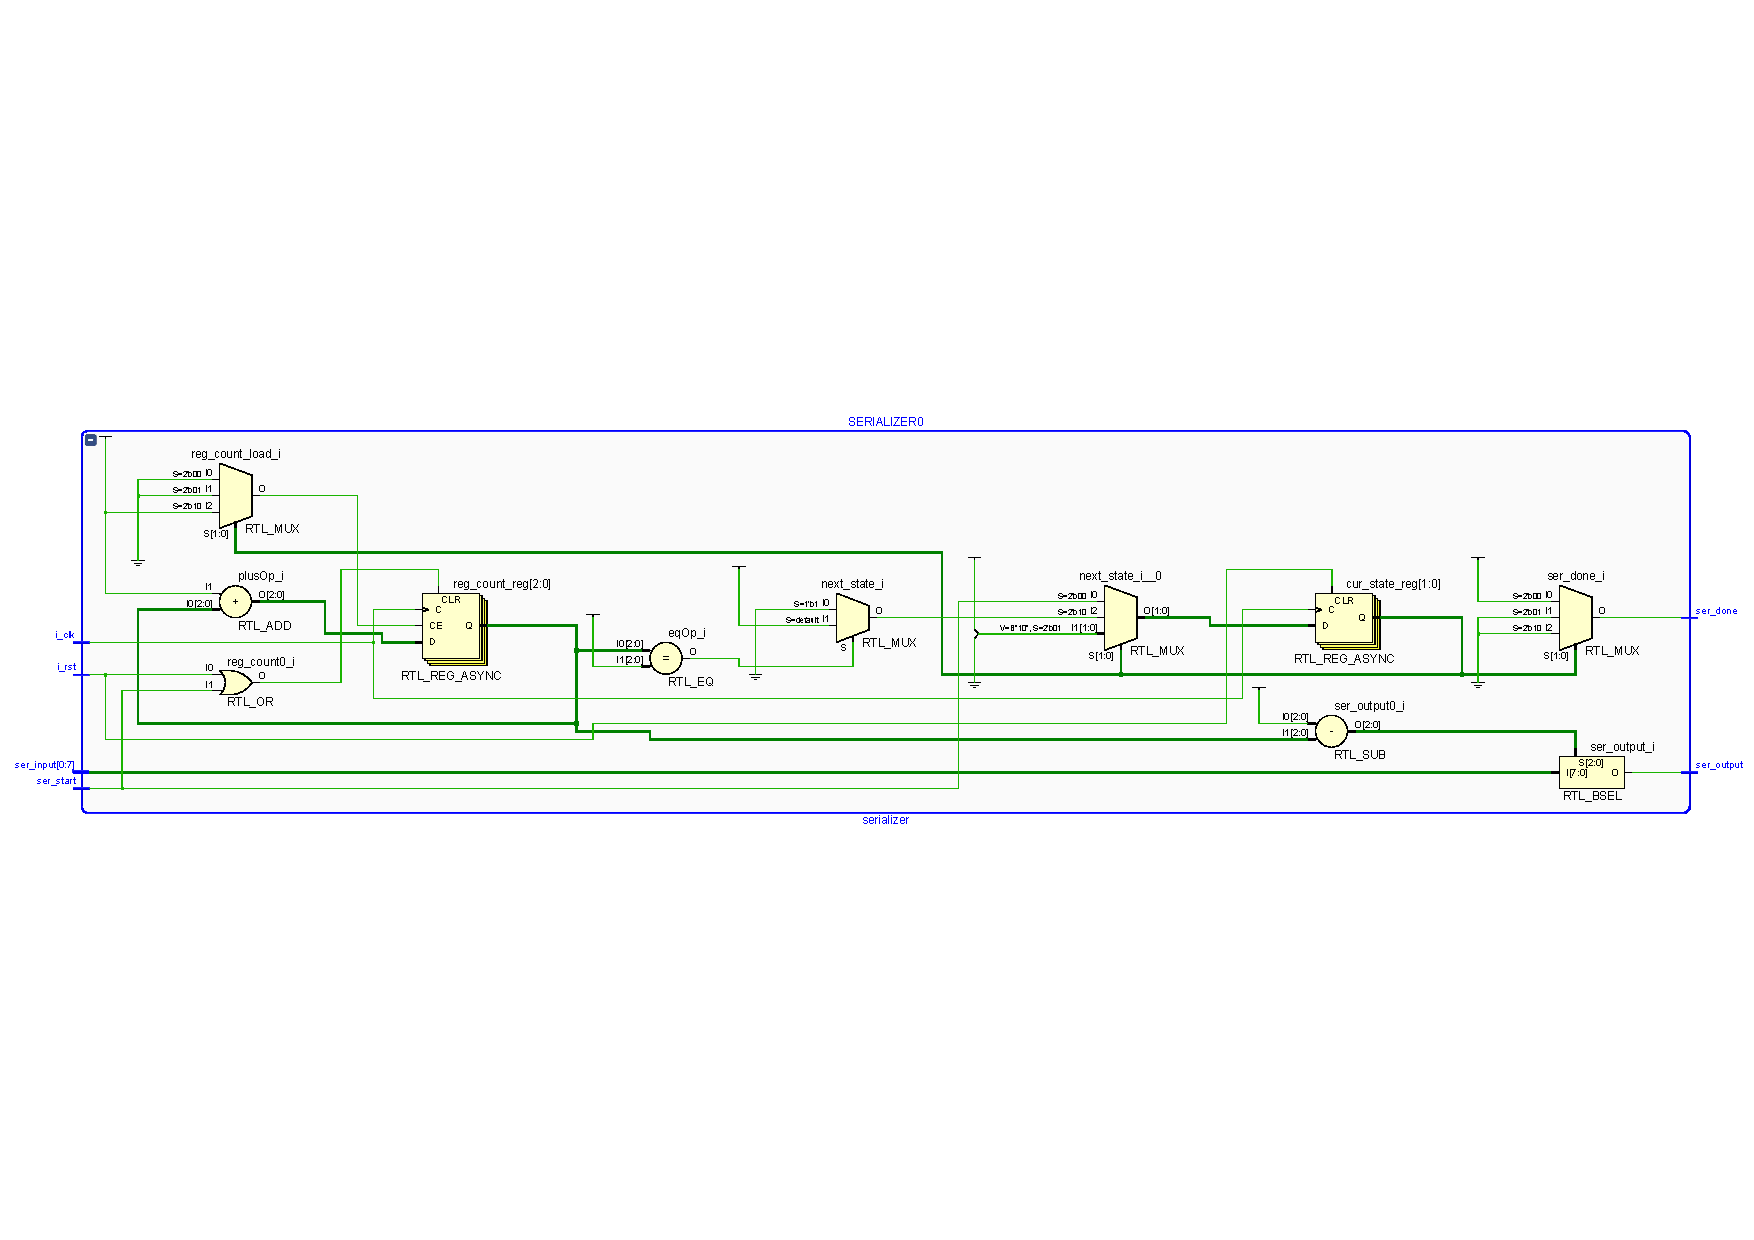
\includegraphics[scale = 0.45]{schematics/serializer.pdf}

\section{Convolutore}
Il \textbf{convolutore} è il componente che emula il comportamento della macchina a stati del convolutore convoluzionale. E' stato realizzato seguendo il modello ad \textit{automa a stati finiti (\textbf{FSM})}.
Il componente si interfaccia (oltre al segnale di \textit{clock} e al segnale di \textit{reset}) a un segnale di reset interno e a un segnale di \textit{pause}. Questo permette al convolutore di fermare la propria macchina a stati ignorando l'\textit{input} ma mantenendo comunque lo stato corrente della macchina. Questo stato di pausa viene utilizzato per attendere i caricamenti da e verso la memoria RAM che richiedono qualche ciclo di clock per caricare/scaricare i registri nella memoria e viceversa. 

L'automa produce due bit in serie per ogni bit ricevuto in ingresso: per questo è fonadmentale che il serializzatore mantenga per due cicli di clock il bit in ingresso. L'automa quindi possiede due stati per ogni macro-stato del convolutore convoluzionale, che corrispondono allo stato in cui l'uscita è settata a pk1 e l'uscita è settata a pk2.

La scelta di implementare il componente in questo modo è stata presa per rispettare le specifiche di progetto:
\begin{displayquote}
  \textit{''Il flusso Y è ottenuto come concatenamento alternato dei due bit di uscita''}
\end{displayquote}

Avendo un convolutore implementato come \textbf{entity separata a sè stante} è possibile utilizzare il componente come da specifica anche in altri progetti. Se per esempio si fosse scelto di gestire l'output del convolutore come una coppia di segnali pk1 e pk2 si sarebbe ridotto il tempo di computazione ma la specifica riguardante il flusso di uscita di dimensione di 1bit sarebbe stata violata.

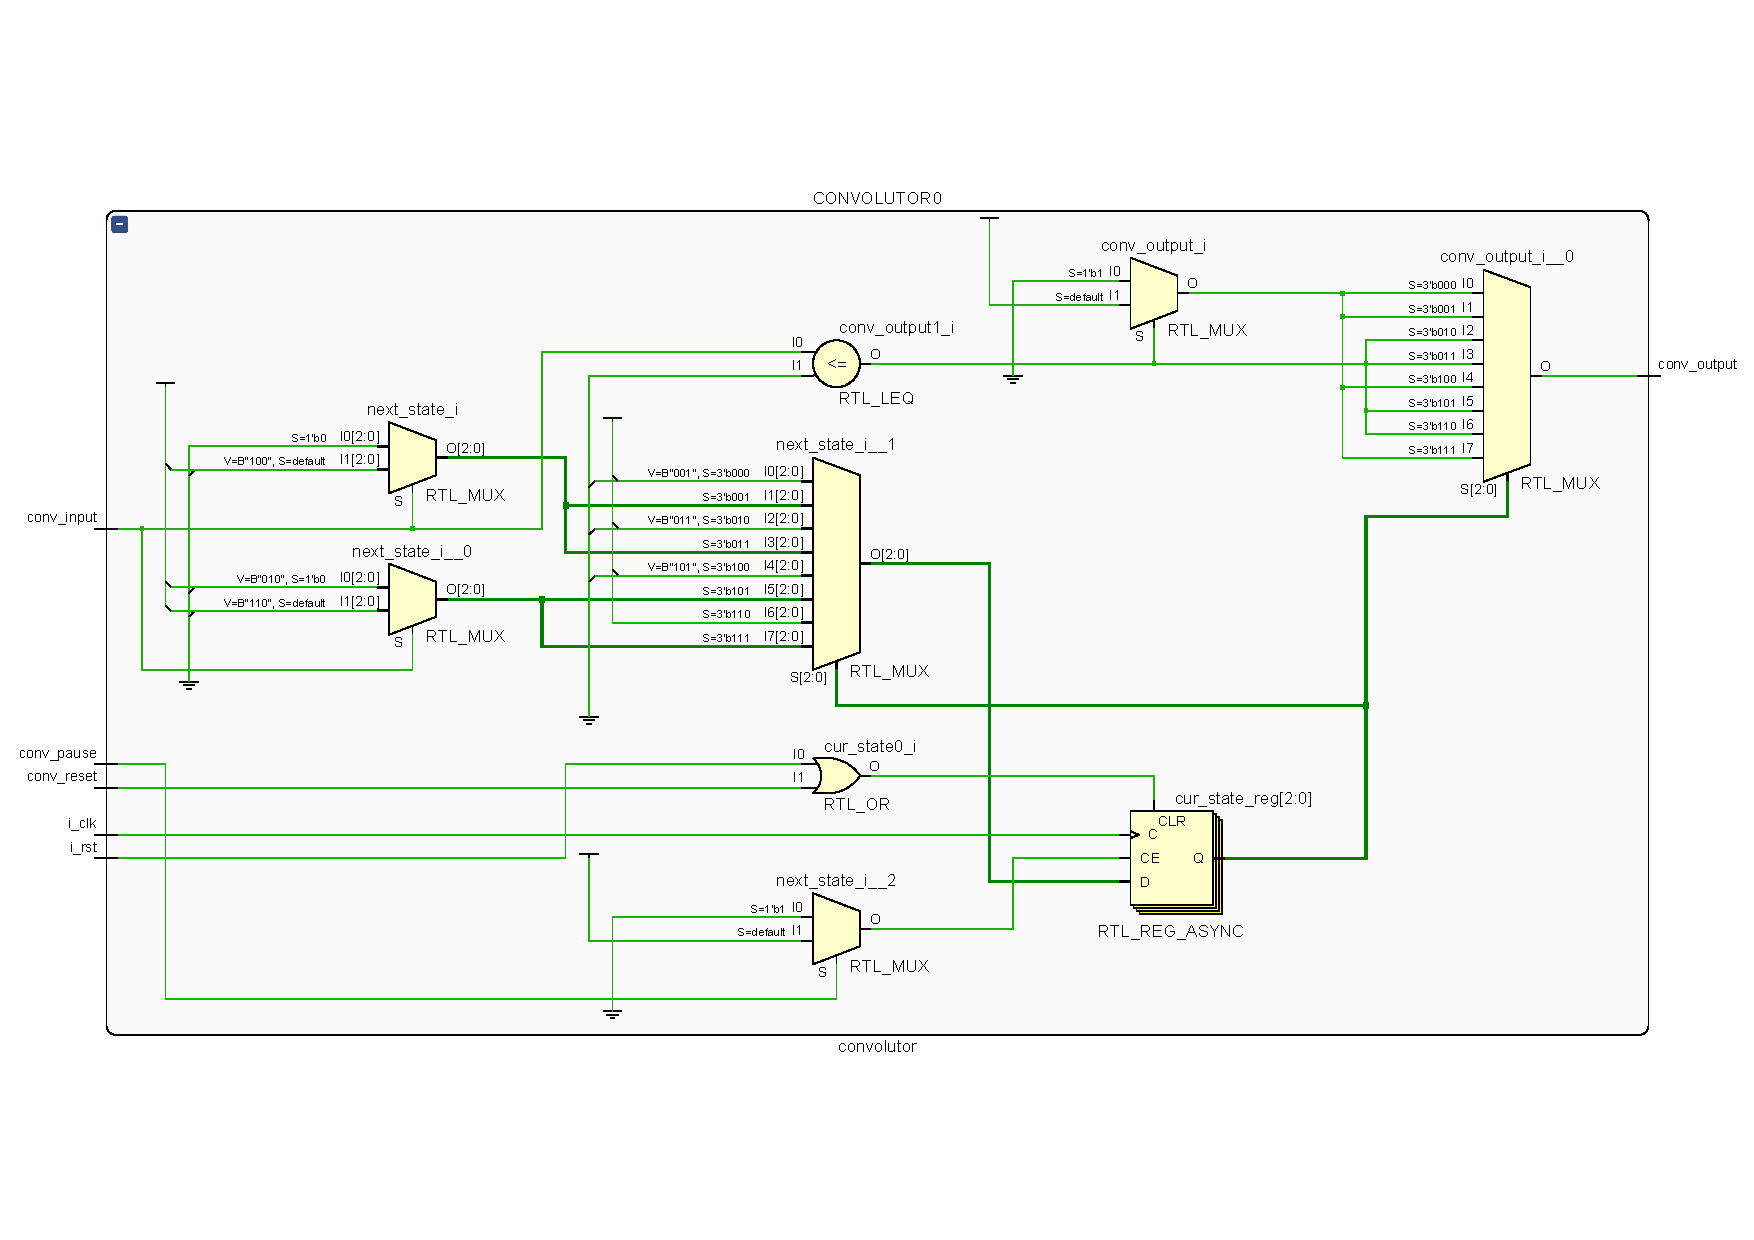
\includegraphics[scale = 0.45]{schematics/convolutor.pdf}

\section{Parallelizzatore}
Il \textbf{parallelizzatore} è il componente addetto alla raccolta del flusso in uscita dal convolutore e alla sua memorizzazione in un registro interno. Questo permette di \textit{impacchettare} il flusso d'uscita in byte in modo da essere scritti sulla memoria ram. 
Dato che per questa configurazione del convolutore a \textbf{ogni byte in ingresso} corrispondono \textbf{2 byte in uscita}, questo componente è stato progettato con un registro interno a \textbf{16 bit} in modo da poter memorizzare i 2 byte in uscita dall'elaborazione di un singolo byte e gestire poi il caricamento delle 2 parole sulla RAM. 

Il parallelizzatore si interfaccia con un ingresso \texttt{[input:1bit]} e produce un'uscita \texttt{[output:8bit]}, selezionabile tramite un \textbf{multiplexer}, che seleziona sull'uscita i bit \texttt{[0-7]} e \texttt{[8-15]} del registro interno.

Al segnale di \texttt{start} il componente passa dallo stato \texttt{STOPPED} allo stato \texttt{ACTIVE}. Quando il componente è attivo memorizza il bit di \textbf{ingresso} nell'\textit{n-esimo} bit del registro interno, incrementando poi il contatore per il prossimo ciclo di clock. La parallelizzazione termina quando il contatore interno raggiunge il valore \texttt{1111}: il registro viene incrementato tornando quindi a \texttt{0} e il parallelizzatore torna nello stato \texttt{STOPPED}, tenendo però comunque memorizzati i valori nel registro. A questo punto la macchina a stati entra negli stati di \textit{caricamento in RAM}, dove carica nel registro di uscita in ordine il primo byte e il secondo nel registro di uscita, da cui poi il dato vene caricato sulla memoria.

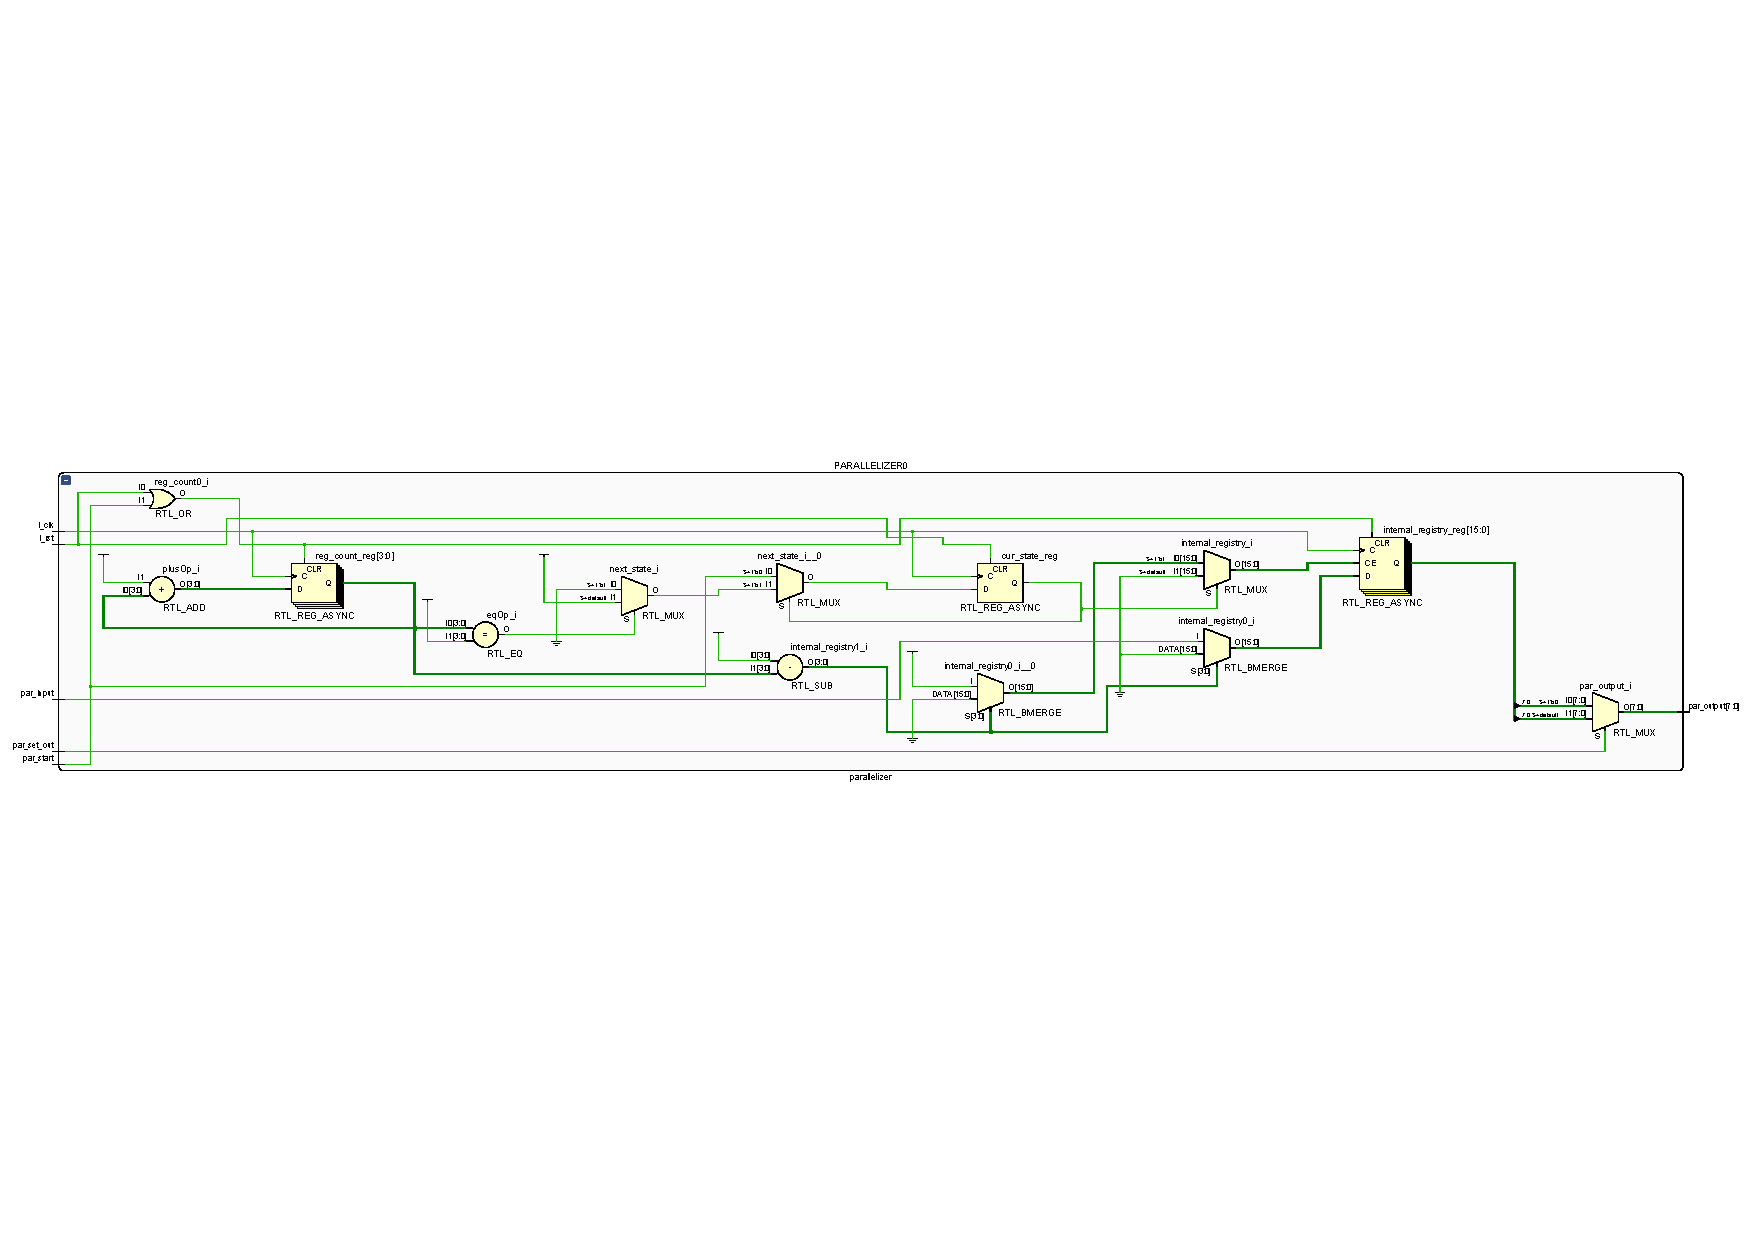
\includegraphics[scale = 0.45]{schematics/parallelizer.pdf}

\section{Datapath}
Il \textbf{datapath} è l'entità che \textbf{fornisce ai vari moduli un'interfaccia} per comunicare tra loro o con la \textbf{memoria RAM}.
Per permettere le comunicazioni tra i vari moduli del dispositivo, istanziati nella macchina a stati (\textit{project\_reti\_logiche}), al datapath sono passati i segnali rappresentanti \textit{dati} (mentre non sono passati quelli di controllo, di responsabilità della macchina a stati) dei vari componenti, che poi vengono connessi all'interno del datapath.

Il datapath contiene inoltre i componenti per interfacciarsi con la RAM e dei registri di supporto per la FSM.
 
\textbf{Registri in out.} Nella fase di lettura dalla memoria ram il dato viene letto e caricato in un registro \textit{reg\_in}. Nella fase di scrittura invece il dato sarà prelevato dal registro \textit{reg\_out}. Entrambi i registri sono da 8bit e sono connessi rispettivamente al serializzatore e al parallelizzatore. Il loro caricamento viene gestito dalla FSM.

\textbf{Registro words.} Nella fase di avvio del dispositivo viene letto all'indirizzo 0 della memoria il numero di byte da cui è formato lo stream di ingresso. Questo valore è memorizzato all'interno del registro \textit{reg\_words}, di 8bit in quanto la dimensione massima dello stream in ingresso è di 255 parole. Il suo caricamento è gestito dalla FSM.

\textbf{Registro count.} Durante l'esecuzione è necessario memorizzare lo stato di avanzamento in modo da sapere a quale indirizzo della RAM accedere per leggere o scrivere dati. Questo resgistro memorizza al suo interno \textit{l'indirizzo} della cella di memoria di \textit{read} a cui si sta puntando. Per esempio se si sta leggendo la terza parola dello stream nel registro sarà presente il valore \texttt{0x0003} in quanto lo stream è memorizzato a partire dall'indirizzo \texttt{0x0001}. E' un registro a 16bit e il suo caricamento e incremento è gestito dalla FSM.

\textbf{Done comparator.} Per rilevare la fine dell'elaborazione nel datapath è presente un comparatore. Esso effettua un controllo che porta un segnale di \textit{done} interno a 1 se il valore contenuto all'interno del registro di \textit{count} supera il numero di parole. Questo sfrutta il fatto che il numero della parola corrente corrisponde al contenuto del registro \textit{count}, in quando l'indirizzo della parola n-esima è n. Inoltre, se dovessimo essere nel caso in cui la lunghezza dello stream fosse 255, il confronto funzionerebbe ancora perchè fino a 255 il processo continuerebbe regolarmente mentre al raggiungimento di 256, valore possibile nel registro degli indirizzi a 16bit \textit{count}, il confronto finirebbe correttamente per segnalare la fine dell'esecuzione.
\begin{verbatim}
  if mux_count <= ("00000000" & reg_words) then
            o_done_signal <= '0';
        else
            o_done_signal <= '1';
\end{verbatim}

\textbf{Multiplexer read write.} Il registro \textit{count} non è direttamente collegato con il segnale \textit{address} della memoria RAM. Questo perchè in scrittura devono essere utilizzati gli indirizzi contigui partendo dall'indirizzo 1000. Questo multiplexer permette di selezionare quale indirizzo viene passato al segnale di indirizzo della memoria:
\begin{verbatim}
  if i_rst = '1' or mux_rw_addr_sel = "00" or mux_rw_addr_sel = "11" then
            o_address <= reg_count;
        elsif mux_rw_addr_sel = "01" then
            o_address <= (mux_count + mux_count) + "0000001111100110";
        else --if mux_rw_addr_sel = "10" then
            o_address <= (mux_count + mux_count) + "0000001111100111";
        end if;
\end{verbatim}
Il mux seleziona di default il contenuto del registro \textit{count} usato in lettura dello stream. Per la scrittura dei due byte corrispondenti all'elaborazione dell'n-esima parola, viene selezionato l'indirizzo $2n + 998$ per il primo byte e $2n + 999$ per il secondo. Questo permette di scrivere nell'indirizzo giusto i due byte derivati dall'elaborazione dell'n-esimo byte. Per esempio, la convoluzione terza parola verrà scritta negli indirizzi \texttt{1004 1005}, in quanto la prima parola è scritta all'interno di \texttt{1000 1001} e la seconda in \texttt{1002 1003}, come da specifica.

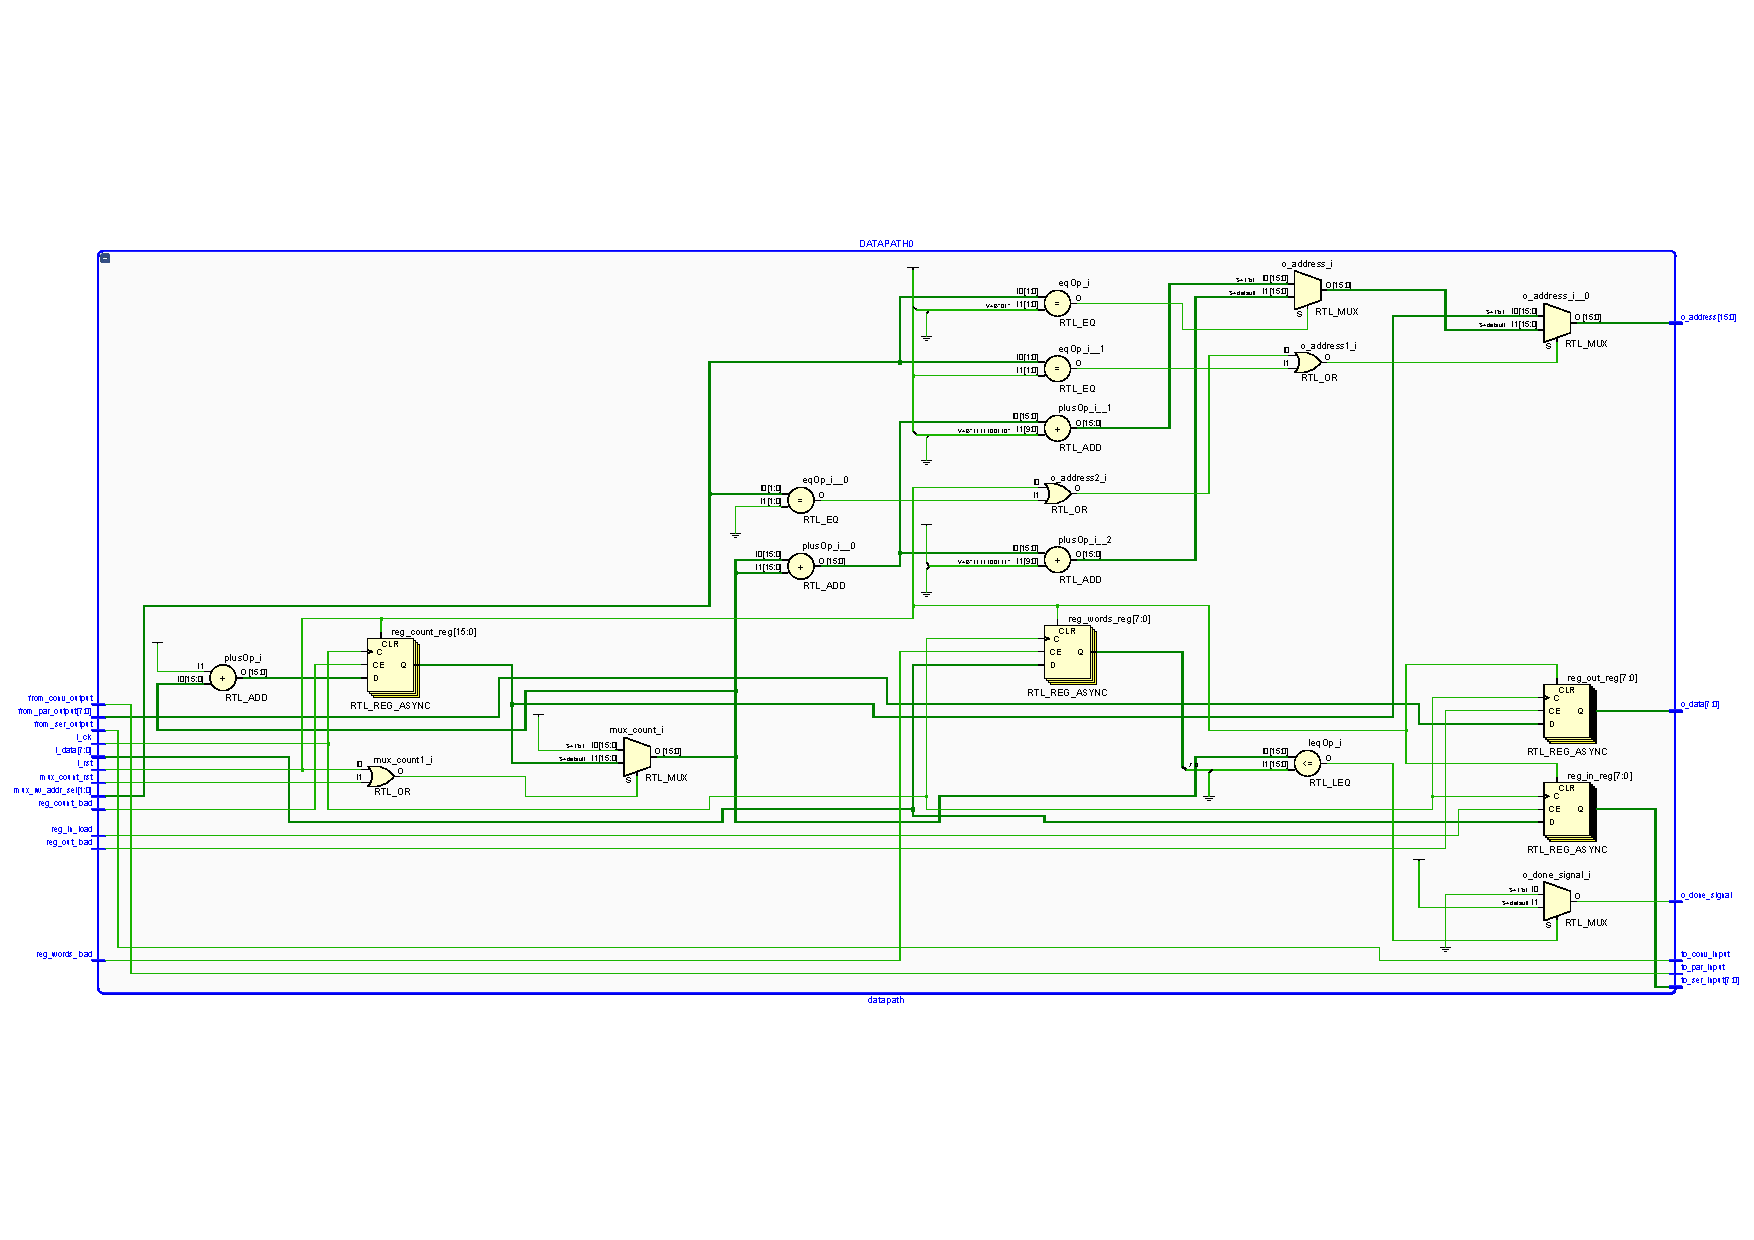
\includegraphics[scale = 0.45]{schematics/datapath.pdf}

\section{Macchina a stati}
Il progetto è tutto contenuto all'interno della entity Vivado \textbf{project\_reti\_logiche}. Questa contiene al suo interno tutti i \textbf{components} del dispositivo (serializer, convolutor, parallelizer e datapath) e implementa tramite tre \textbf{process} (\textit{FSM\_STATE\_CHANGE, FSM\_FLOW, FSM\_OUT}). Questa FSM permette di controllare il flusso d'esecuzione di tutto il dispositivo portando i segnali di controllo ai valori corretti in base allo stato in cui ci si trova.

\subsection{Elenco delle transizioni}
Segue un elenco delle transizioni. Vedi figura \ref{fig:FSM Flow}
\begin{verbatim}
RESET                   => i_start            ? READ_WORD_RAM_REQUEST : RESET
READ_WORDS_RAM_REQUEST  => READ_WORDS_RAM_READ
READ_WORDS_RAM_READ     => READ_RAM_REQUEST
READ_RAM_REQUEST        => o_done_signal      ? DONE : READ_RAM
READ_RAM                => SERIALIZE
SERIALIZE               => ser_done           ? LOAD_FROM_PAR : SERIALIZE
LOAD_FROM_PAR           => WRITE_RAM_1        
WRITE_RAM_1             => WRITE_RAM_2
WRITE_RAM_2             => WRITE_RAM_WAIT
WRITE_RAM_WAIT          => READ_RAM_REQUEST
DONE                    => i_start            ? DONE : RESET
\end{verbatim}


\begin{figure}[h] % ’ht’ tells LaTeX to place the figure ’here’ or at the top of the page
  \newpage
  \centering % centers the figure
  \begin{tikzpicture} [state/.style={circle, draw, minimum size=2.3cm, thick, font=\small, fill=gray!10}]
    \node[state, initial] (RESET) {$RESET$};
    \node[state, right of=RESET] (READ_WORDS_RAM_REQUEST) {$RWR\_REQ$};
    \node[state, right of=READ_WORDS_RAM_REQUEST] (READ_WORDS_RAM_READ) {$RWR\_READ$};
    \node[state, below of=READ_WORDS_RAM_READ] (READ_RAM_REQUEST) {$RR\_REQ$};
    \node[state, below of=READ_RAM_REQUEST] (READ_RAM) {$READ\_RAM$};
    \node[state, below of=READ_RAM] (SERIALIZE) {$SERIALIZE$};
    \node[state, below of=SERIALIZE] (LOAD_FROM_PAR) {$LOAD\_PAR$};
    \node[state, left of=LOAD_FROM_PAR] (WRITE_RAM_1) {$WRAM\_1$};
    \node[state, left of=WRITE_RAM_1] (WRITE_RAM_2) {$WRAM\_2$};
    \node[state, above of=WRITE_RAM_2] (WRITE_RAM_WAIT) {$WR\_WAIT$};
    \node[state, below of=RESET] (DONE) {$DONE$};
    
    \draw (RESET) edge[loop above] node{$i\_start = 0$} (RESET)
          (RESET) edge[above] node{$i\_start = 1$} (READ_WORDS_RAM_REQUEST)
          
          (READ_WORDS_RAM_REQUEST) edge[above] node{} (READ_WORDS_RAM_READ)
          (READ_WORDS_RAM_READ) edge[above] node{} (READ_RAM_REQUEST)

          (READ_RAM_REQUEST) edge[above] node {$o\_done\_signal = 1$} (DONE)
          (READ_RAM_REQUEST) edge[above] node[right]{$o\_done\_signal = 0$} (READ_RAM)

          (READ_RAM) edge[above] node{} (SERIALIZE)

          (SERIALIZE) edge[loop left] node{$ser\_done = 0$} (SERIALIZE)
          (SERIALIZE) edge[above] node[right]{$ser\_done = 1$} (LOAD_FROM_PAR)

          (LOAD_FROM_PAR) edge[above] node{} (WRITE_RAM_1)
          (WRITE_RAM_1) edge[above] node{} (WRITE_RAM_2)
          (WRITE_RAM_2) edge[above] node{} (WRITE_RAM_WAIT)
          (WRITE_RAM_WAIT) edge[bend left] node{} (READ_RAM_REQUEST)

          (DONE) edge[loop left] node{$i\_start=1$} (DONE)
          (DONE) edge[above] node[left]{$i\_start=0$} (RESET)
          ;
  \end{tikzpicture}
  \caption{FSM Flow}
  \label{fig:FSM Flow}
\end{figure}

\subsection{Descrizione degli stati}
La macchina a stati è modellata come una macchina di Moore. I segnali di controllo sono dipendenti solamente dallo stato corrente della macchina. In seguito sono elencate le uscite dei segnali di controllo per ogni stato. Di default tutti gli stati sono portati al livello logico basso.

\subsubsection{RESET}
Lo stato di reset corrisponde allo stato iniziale della macchina. La macchina torna in questo stato alla fine di una computazione quando è stato riabbassato il segnale di start o quando il segnale di reset è portato a 1.

In questo stato si azzera il registro count degli indirizzi tramite un multiplexer e si azzera lo stato del convolutore, riportandolo nello stato iniziale in modo da poter iniziare una elaborazione sempre con il convolutore azzerato anche in caso di multiple elaborazioni in sequenza.

Si esce dallo stato di reset non appena una nuova elaborazione è richiesta tramite il segnale di start.

\begin{table}[H]
  \centering
  \begin{tabular}{||c | c||} 
    \hline
    Signal & Value \\
    \hline\hline
    reg\_in\_load & 0 \\
    reg\_out\_load & 0 \\
    reg\_words\_load & 0 \\
    \textbf{reg\_count\_load} & \textbf{1} \\
    \textbf{mux\_count\_rst} & \textbf{1} \\
    mux\_rw\_addr\_sel & 00 \\
    ser\_start & 0 \\
    \textbf{conv\_reset} & \textbf{1} \\
    par\_set\_out & 0 \\
    o\_en & 0 \\
    o\_we & 0 \\
    o\_done & 0 \\
   \hline
  \end{tabular}
  \caption{Uscite nello stato RESET.}
  \label{table:1}
\end{table}


\subsubsection{READ\_WORDS\_RAM\_REQUEST}
Nello stato di READ\_WORDS\_RAM\_REQUEST si carica all'interno del registro words il numero di byte corrispondente alla lunghezza dello stream in input. Questo valore viene richiesto alla RAM in questo stato.
\begin{table}[H]
  \centering
  \begin{tabular}{||c | c||} 
    \hline
    Signal & Value \\
    \hline\hline
    reg\_in\_load & 0 \\
    reg\_out\_load & 0 \\
    reg\_words\_load & 0 \\
    reg\_count\_load & 0 \\
    mux\_count\_rst & 0 \\
    \textbf{mux\_rw\_addr\_sel} & \textbf{00} \\
    ser\_start & 0 \\
    conv\_reset & 0 \\
    par\_set\_out & 0 \\
    \textbf{o\_en} & \textbf{1} \\
    o\_we & 0 \\
    o\_done & 0 \\
   \hline
  \end{tabular}
  \caption{Uscite nello stato READ\_WORDS\_RAM\_REQUEST.}
  \label{table:2}
\end{table}

\subsubsection{READ\_WORDS\_RAM\_READ}
Essendo la memoria sincrona, essa rilasia il dato richiesto al ciclo di clock precedente solamente durante quello successivo. In questo stato, raggiunto nel ciclo di clock immediatamente successivo al ciclo dello stato READ\_WORDS\_RAM\_REQUEST, si carica il valore recuperato dalla RAM all'interno del registro \textit{words}.
\begin{table}[H]
  \centering
  \begin{tabular}{||c | c||} 
    \hline
    Signal & Value \\
    \hline\hline
    reg\_in\_load & 0 \\
    reg\_out\_load & 0 \\
    \textbf{reg\_words\_load} & \textbf{1} \\
    \textbf{reg\_count\_load} & \textbf{1} \\
    mux\_count\_rst & 0 \\
    mux\_rw\_addr\_sel & 00 \\
    ser\_start & 0 \\
    conv\_reset & 0 \\
    par\_set\_out & 0 \\
    o\_en & 0 \\
    o\_we & 0 \\
    o\_done & 0 \\
   \hline
  \end{tabular}
  \caption{Uscite nello stato READ\_WORDS\_RAM\_READ.}
  \label{table:3}
\end{table}

\subsubsection{READ\_RAM\_REQUEST}
READ\_RAM\_REQUEST è lo stato che richiede alla memoria RAM il byte dello stream da leggere per proseguire con l'elaborazione. Per questo utilizza il mux di selettore indirizzo a 00 in modo da andare a leggere dall'indirizzo di lettura già contenuto nel registro di count. 

Oltre all'interrogaizone della RAM lo stato effettua una funzione di controllo: se dal datapth arriva il segnale \textit{o\_done\_signal} il prossimo stato non sarà quello di caricamento nel registro in della parola letta dalla memoria ma lo stato di DONE, dove viene notificata la fine dell'elaborazione.

\begin{table}[H]
  \centering
  \begin{tabular}{||c | c||} 
    \hline
    Signal & Value \\
    \hline\hline
    reg\_in\_load & 0 \\
    reg\_out\_load & 0 \\
    reg\_words\_load & 0 \\
    reg\_count\_load & 0 \\
    mux\_count\_rst & 0 \\
    \textbf{mux\_rw\_addr\_sel} & \textbf{00} \\
    ser\_start & 0 \\
    conv\_reset & 0 \\
    par\_set\_out & 0 \\
    \textbf{o\_en} & \textbf{1} \\
    o\_we & 0 \\
    o\_done & 0 \\
   \hline
  \end{tabular}
  \caption{Uscite nello stato READ\_RAM\_REQUEST.}
  \label{table:4}
\end{table}

\subsubsection{READ\_RAM}
In questo stato il byte dello stream richiesto al ciclo precedente viene letto e caricato all'interno del registro \textit{reg\_in}. Inoltre è alzato il segnale di start del serializzatore in modo da far partire l'elaborazione nel ciclo successivo.

\begin{table}[H]
  \centering
  \begin{tabular}{||c | c||} 
    \hline
    Signal & Value \\
    \hline\hline
    \textbf{reg\_in\_load} & \textbf{1} \\
    reg\_out\_load & 0 \\
    reg\_words\_load & 0 \\
    reg\_count\_load & 0 \\
    mux\_count\_rst & 0 \\
    mux\_rw\_addr\_sel & 00 \\
    \textbf{ser\_start} & \textbf{1} \\
    conv\_reset & 0 \\
    par\_set\_out & 0 \\
    o\_en & 0 \\
    o\_we & 0 \\
    o\_done & 0 \\
   \hline
  \end{tabular}
  \caption{Uscite nello stato READ\_RAM.}
  \label{table:5}
\end{table}

\subsubsection{SERIALIZE}
Nello stato serialize avviene tutto il calcolo della convoluzione del byte presente all'interno del registro \textit{reg\_in}. Il serializzatore continua finchè non ha serializzato tutto il registro \textit{reg\_in}, quando alzerà il segnale \textit{ser\_done}, che mette in pausa il convolutore. Il parallelizzatore, partito anch'esso con il segnale di \textit{ser\_start} sarà valido alla fine della convoluzione del byte. Quando il segnale di \textit{ser\_done} è alzato dopo 16 cicli di clock si passa alla sezione di caricamento in RAM.
\begin{table}[H]
  \centering
  \begin{tabular}{||c | c||} 
    \hline
    Signal & Value \\
    \hline\hline
    reg\_in\_load & 0 \\
    reg\_out\_load & 0 \\
    reg\_words\_load & 0 \\
    reg\_count\_load & 0 \\
    mux\_count\_rst & 0 \\
    mux\_rw\_addr\_sel & 00 \\
    ser\_start & 0 \\
    conv\_reset & 0 \\
    par\_set\_out & 0 \\
    o\_en & 0 \\
    o\_we & 0 \\
    o\_done & 0 \\
   \hline
  \end{tabular}
  \caption{Uscite nello stato SERIALIZE.}
  \label{table:6}
\end{table}

\subsubsection{LOAD\_FROM\_PAR}
In questo stato si carica dal registro interno del parallelizzatore al registro di uscita \textit{reg\_out} il primo byte da scrivere in memoria. Il byte corretto viene selezionato mandando al parallelizzatore il bit di comando del suo mux di uscita. Il primo byte viene selezionato con il segnale 0.

\begin{table}[H]
  \centering
  \begin{tabular}{||c | c||} 
    \hline
    Signal & Value \\
    \hline\hline
    reg\_in\_load & 0 \\
    \textbf{reg\_out\_load} & \textbf{1} \\
    reg\_words\_load & 0 \\
    reg\_count\_load & 0 \\
    mux\_count\_rst & 0 \\
    mux\_rw\_addr\_sel & 00 \\
    ser\_start & 0 \\
    conv\_reset & 0 \\
    \textbf{par\_set\_out} & \textbf{0} \\
    o\_en & 0 \\
    o\_we & 0 \\
    o\_done & 0 \\
   \hline
  \end{tabular}
  \caption{Uscite nello stato LOAD\_FROM\_PAR.}
  \label{table:7}
\end{table}

\subsubsection{WRITE\_RAM\_1}
Nel primo stato di scrittura viene richiesta alla RAM la scrittura del primo byte, presente già nel registro di uscita. Questo viene scrito all'indirizzo selezionato con il mux di indirizzo a 01. Inoltre sempre durante questo stato viene richiesto il caricamento del secondo byte in ingresso nel registro di out, in modo da averlo già caricato per il successivo ciclo di clock e richiedere già la sua scrittura.
\begin{table}[H]
  \centering
  \begin{tabular}{||c | c||} 
    \hline
    Signal & Value \\
    \hline\hline
    reg\_in\_load & 0 \\
    \textbf{reg\_out\_load} & \textbf{1} \\
    reg\_words\_load & 0 \\
    reg\_count\_load & 0 \\
    mux\_count\_rst & 0 \\
    \textbf{mux\_rw\_addr\_sel} & \textbf{01} \\
    ser\_start & 0 \\
    conv\_reset & 0 \\
    \textbf{par\_set\_out} & \textbf{1} \\
    \textbf{o\_en} & \textbf{1} \\
    \textbf{o\_we} & \textbf{1} \\
    o\_done & 0 \\
   \hline
  \end{tabular}
  \caption{Uscite nello stato WRITE\_RAM\_1.}
  \label{table:8}
\end{table}

\subsubsection{WRITE\_RAM\_2}
In questo stato, come nel precedente, viene richiesta la scrittura del registro di output, che in questo ciclo di clock avrà caricato il secondo byte presente nel parallelizzatore. Per il secondo byte viene scelto l'indirizzo selezionato 10 dal mux degli indirizzi.
\begin{table}[H]
  \centering
  \begin{tabular}{||c | c||} 
    \hline
    Signal & Value \\
    \hline\hline
    reg\_in\_load & 0 \\
    reg\_out\_load & 0 \\
    reg\_words\_load & 0 \\
    reg\_count\_load & 0 \\
    mux\_count\_rst & 0 \\
    \textbf{mux\_rw\_addr\_sel} & \textbf{10} \\
    ser\_start & 0 \\
    conv\_reset & 0 \\
    par\_set\_out & 0 \\
    \textbf{o\_en} & \textbf{1} \\
    \textbf{o\_we} & \textbf{1} \\
    o\_done & 0 \\
   \hline
  \end{tabular}
  \caption{Uscite nello stato WRITE\_RAM\_2.}
  \label{table:9}
\end{table}

\subsubsection{WRITE\_RAM\_WAIT}
Durante questo ciclo di clock la RAM sta completando il caricamento del secondo byte dello stream di uscita. Con questo stato di attesa si aspetta in modo da avere una RAM valida già in uscita da questo stato. Inoltre si incrementa il counter degli indirizzi in modo che il prossimo stato (READ\_RAM\_REQUEST) abbia il contatore aggiornato e possa svolgere la verifica dello stato dell'elaborazione.
\begin{table}[H]
  \centering
  \begin{tabular}{||c | c||} 
    \hline
    Signal & Value \\
    \hline\hline
    reg\_in\_load & 0 \\
    reg\_out\_load & 0 \\
    reg\_words\_load & 0 \\
    \textbf{reg\_count\_load} & \textbf{1} \\
    mux\_count\_rst & 0 \\
    mux\_rw\_addr\_sel & 00 \\
    ser\_start & 0 \\
    conv\_reset & 0 \\
    par\_set\_out & 0 \\
    o\_en & 0 \\
    o\_we & 0 \\
    o\_done & 0 \\
   \hline
  \end{tabular}
  \caption{Uscite nello stato WRITE\_RAM\_WAIT.}
  \label{table:10}
\end{table}

\subsubsection{DONE}
Questo è lo stato di fine elaborazione. Esso porta il segnale \textit{o\_done} a alto. Si resta in questo stato fintantochè il segnale di start non viene riabbassato dall'utente. A quel punto la macchina tornerà nello stati iniziale (RESET) abbassando il segnale di done e rendendolo prondo per una nuova elaborazione, come da specifica.
\begin{table}[H]
  \centering
  \begin{tabular}{||c | c||} 
    \hline
    Signal & Value \\
    \hline\hline
    reg\_in\_load & 0 \\
    reg\_out\_load & 0 \\
    reg\_words\_load & 0 \\
    reg\_count\_load & 0 \\
    mux\_count\_rst & 0 \\
    mux\_rw\_addr\_sel & 00 \\
    ser\_start & 0 \\
    conv\_reset & 0 \\
    par\_set\_out & 0 \\
    o\_en & 0 \\
    o\_we & 0 \\
    \textbf{o\_done} & \textbf{1} \\
   \hline
  \end{tabular}
  \caption{Uscite nello stato DONE.}
  \label{table:11}
\end{table}

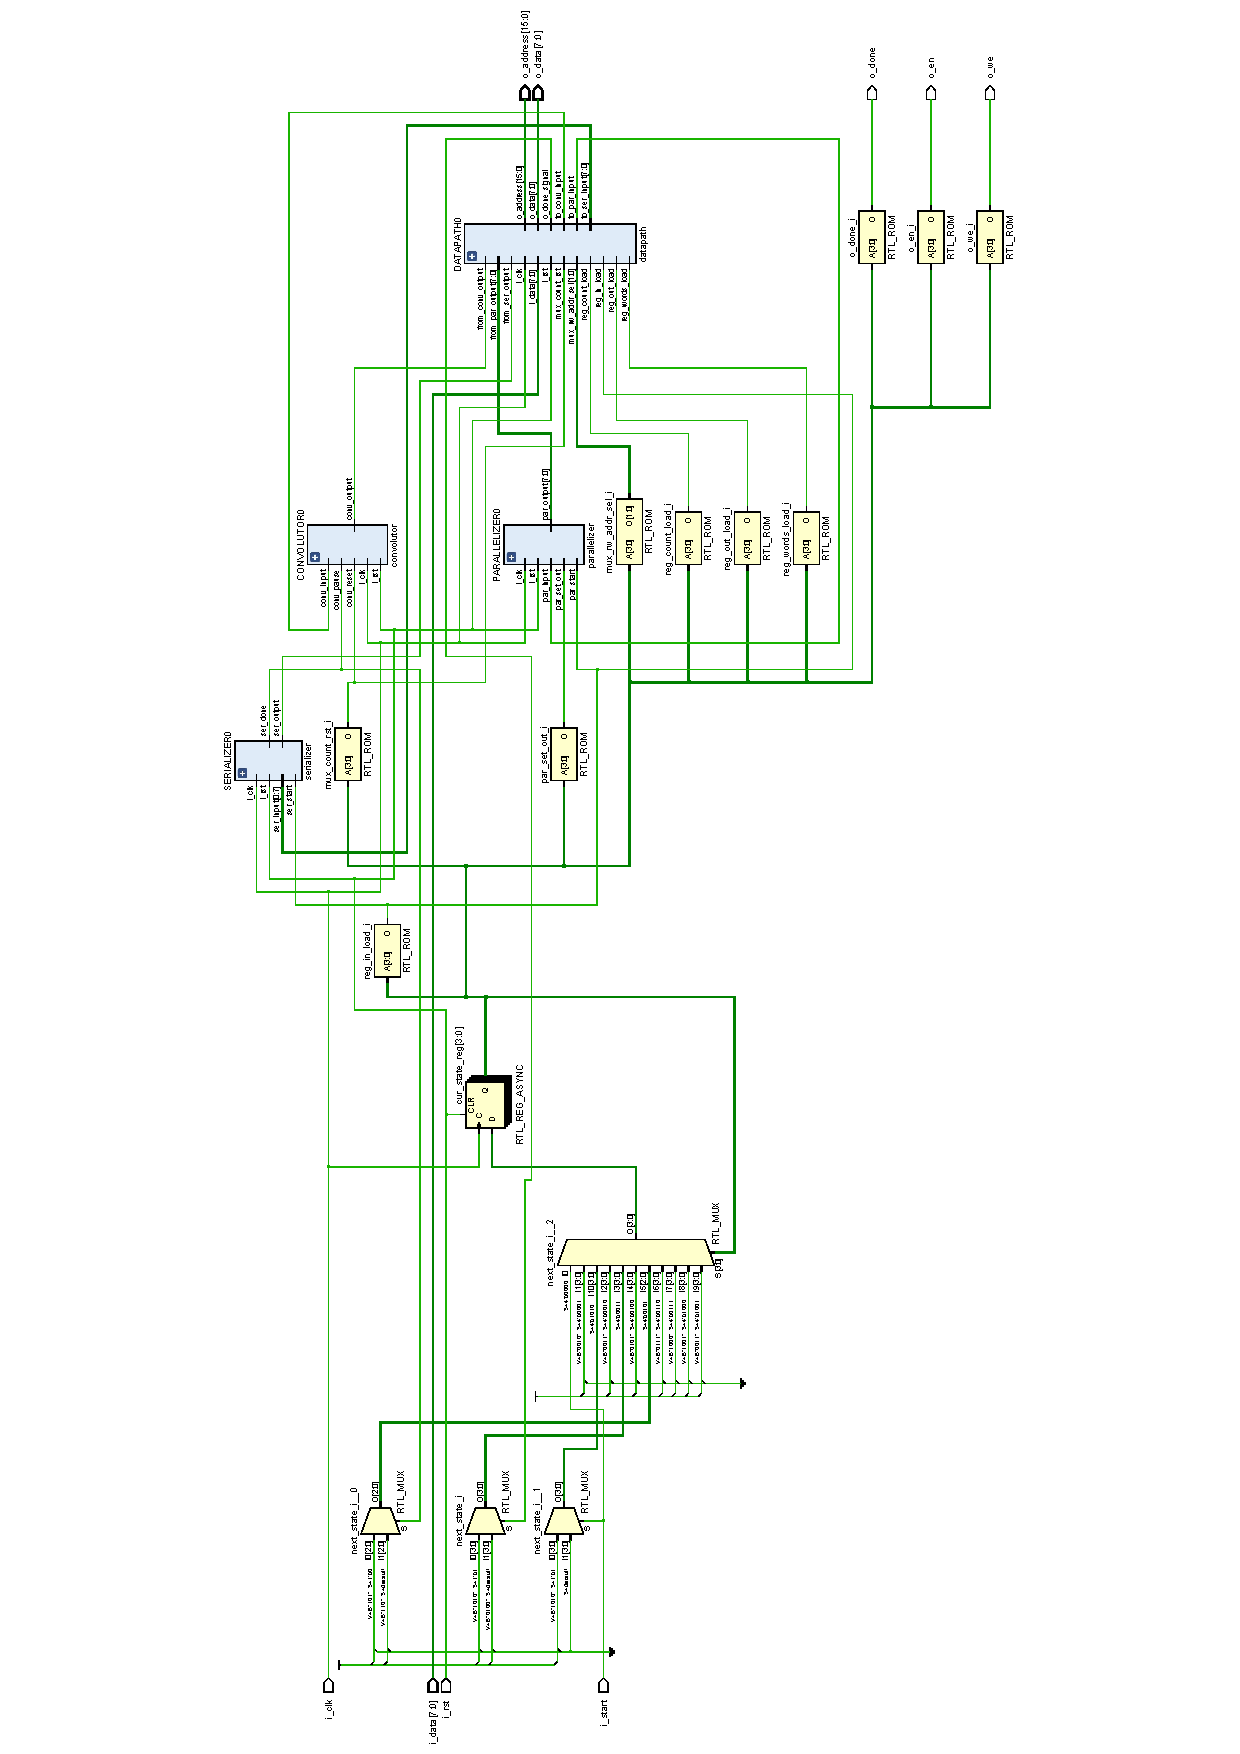
\includegraphics[scale = 0.45]{schematics/schematic.pdf}
\\
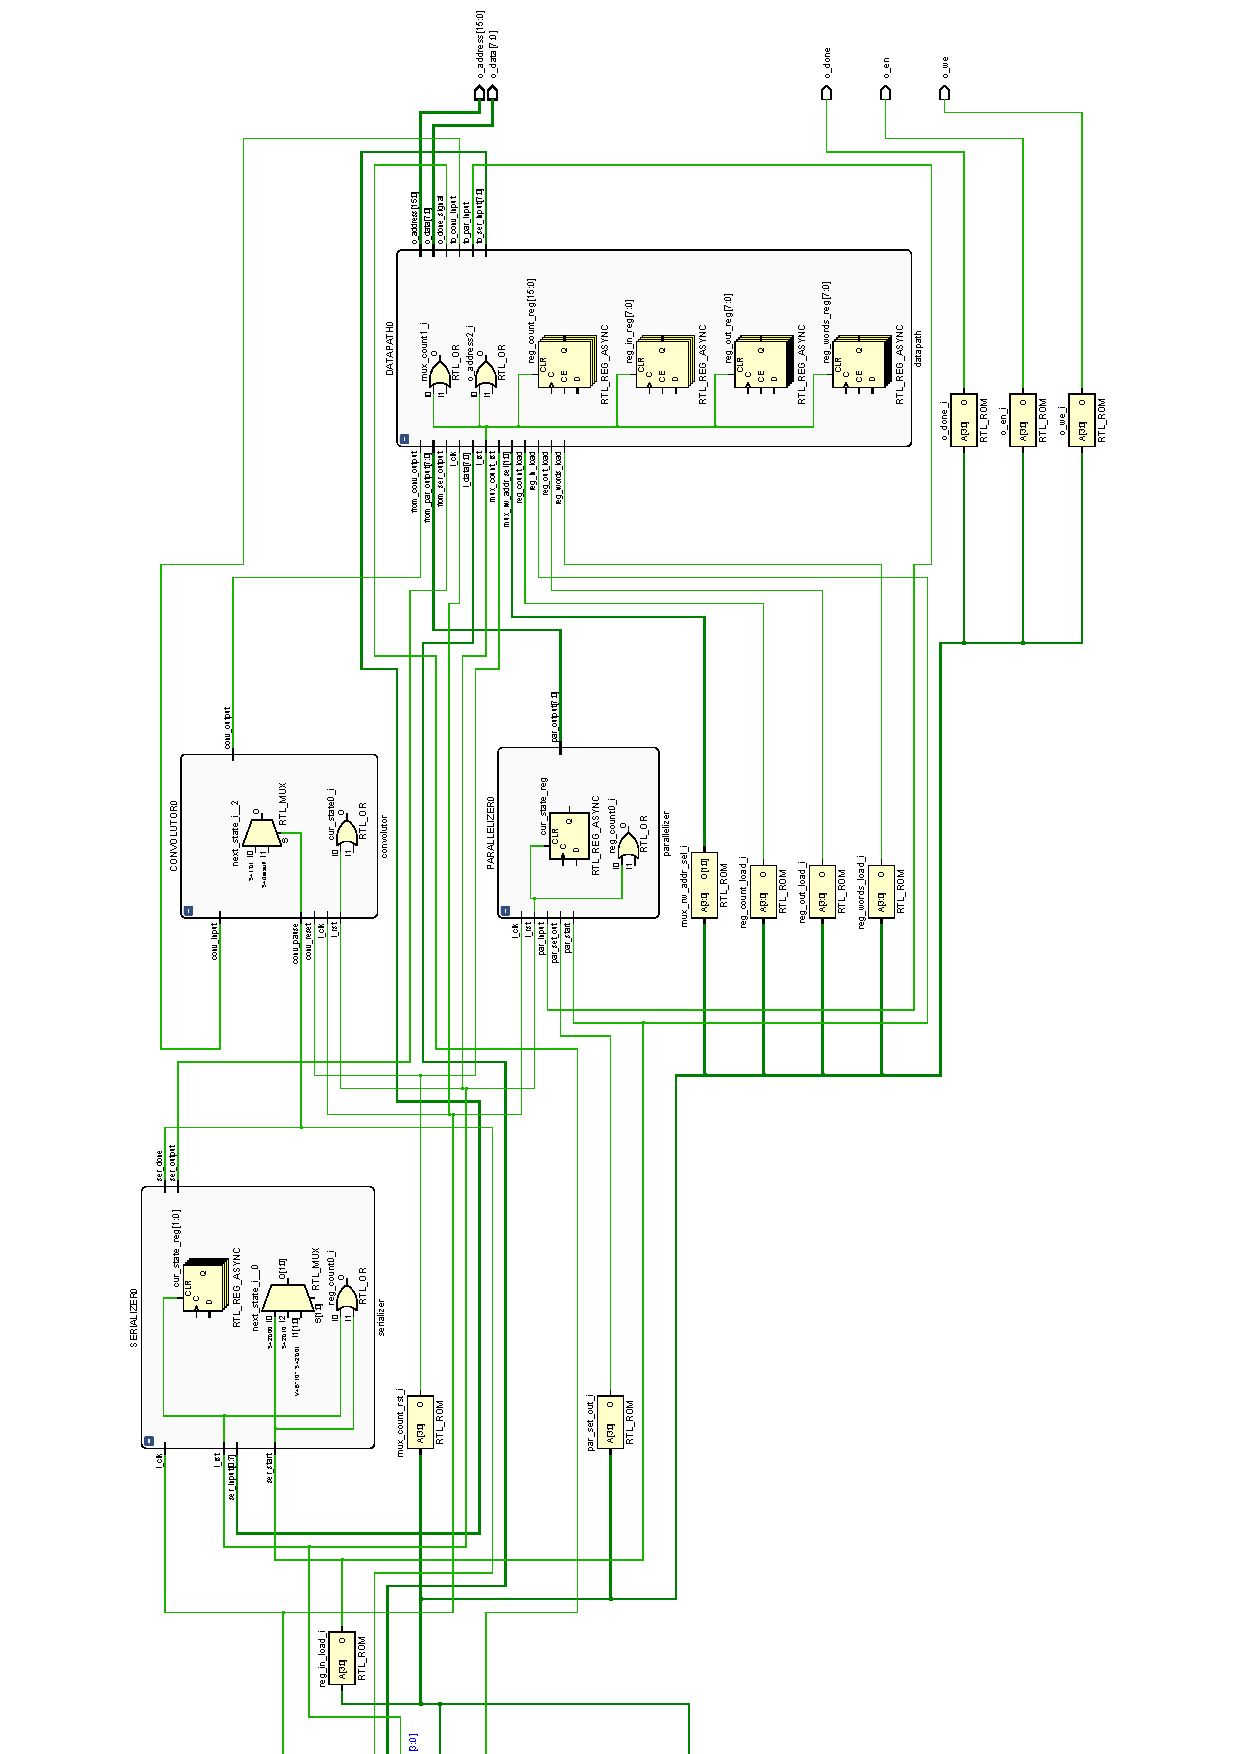
\includegraphics[scale = 0.45]{schematics/schematicComplete.pdf}

%----------------------------------------------------------------------------------------
%	RISULTATI SPERIMENTALI
%----------------------------------------------------------------------------------------

\chapter{Risultati sperimentali}
Il dispositivo progettato è stato sintetizzato e testato con il tool Vivado di Xilinx. Vengono riportate ora le analisi sugli aspetti di sintesi del dispositivo e sui test effettuati su di esso.

\section{Sintesi}
La sintesi è eseguita con un constraint sul periodo di clock di \textbf{100ns} e con una fpga target \textbf{FPGA Artix 7 \texttt{xc7a200tfbg484-1}}.
\subsection{Componenti}
Il report di sintesi riassume l'elenco dei componenti della FPGA utilizzati per sintetizzare il dispositivo.

\begin{verbatim}
+-------------------------+------+-------+------------+-----------+-------+
|        Site Type        | Used | Fixed | Prohibited | Available | Util% |
+-------------------------+------+-------+------------+-----------+-------+
| Slice LUTs*             |  109 |     0 |          0 |    134600 |  0.08 |
|   LUT as Logic          |  109 |     0 |          0 |    134600 |  0.08 |
|   LUT as Memory         |    0 |     0 |          0 |     46200 |  0.00 |
| Slice Registers         |   81 |     0 |          0 |    269200 |  0.03 |
|   Register as Flip Flop |   81 |     0 |          0 |    269200 |  0.03 |
|   Register as Latch     |    0 |     0 |          0 |    269200 |  0.00 |
| F7 Muxes                |    1 |     0 |          0 |     67300 | <0.01 |
| F8 Muxes                |    0 |     0 |          0 |     33650 |  0.00 |
+-------------------------+------+-------+------------+-----------+-------+
\end{verbatim}

Si può notare come tutti i registri utilizzati siano    \textbf{sincroni} (flip flop).

\subsection{Timing}
Il report di timing riassume i parametri della scheda in relazione al segnale di clock

\begin{verbatim}
Slack (MET) :             95.783ns  (required time - arrival time)
  Source:                 DATAPATH0/reg_count_reg[3]/C
                            {rise@0.000ns fall@50.000ns period=100.000ns}
  Destination:            FSM_onehot_cur_state_reg[4]/D
                            {rise@0.000ns fall@50.000ns period=100.000ns}
  Path Group:             clock
  Path Type:              Setup (Max at Slow Process Corner)
  Requirement:            100.000ns  (clock rise@100.000ns - clock rise@0.000ns)
  Data Path Delay:        4.066ns  (logic 1.496ns (36.793%)  route 2.570ns (63.207%))
  Logic Levels:           4  (CARRY4=2 LUT4=1 LUT6=1)
  Clock Path Skew:        -0.145ns (DCD - SCD + CPR)
    Destination Clock Delay (DCD):    2.100ns = ( 102.100 - 100.000 ) 
    Source Clock Delay      (SCD):    2.424ns
    Clock Pessimism Removal (CPR):    0.178ns
  Clock Uncertainty:      0.035ns  ((TSJ^2 + TIJ^2)^1/2 + DJ) / 2 + PE
    Total System Jitter     (TSJ):    0.071ns
    Total Input Jitter      (TIJ):    0.000ns
    Discrete Jitter          (DJ):    0.000ns
    Phase Error              (PE):    0.000ns
\end{verbatim}

Si può notare come lo \textbf{slack} (parametro che indica il tempo tra il delay massimo della logica combinatoria e il prossimo rising-edge del ciclo di clock) sia particolarmente elevato. Questo a grazie al delay della logica combinatoria (\textbf{4.066ns}) che risulta più di un ordine di grandezza inferiore al periodo del ciclo di clock (100ns).
Questo dato indica quindi che la scheda sarebbe in grado di girare a 10 volte la velocità attuale, ovvero con un ciclo di clock di periodo 10ns (100Mhz).

%----------------------------------------------------------------------------------------
%	CONCLUSIONE
%----------------------------------------------------------------------------------------

\chapter{Conclusione}


\end{document}